\section[NFC \& RFID]{Near Field Communication (NFC) \& Radio Frequency Identification (RFID)}
\begin{mytitle}[RFID] RFID identifies objects from a distance. It is a small integrated circuit with a radio frequency transponder. A transponder is a transmitter-responder which generates a response to a received signal. The RFID circuit runs on a wireless energy supply due to a magnetic or electromagnetic field. It contains around 100 Bytes of ROM or EEPROM and costs around 1 cent.
\end{mytitle}
\begin{mytitle}[Performance of RFID chips]\hfill
\begin{itemize}
    \item Low end features: read-only memory, tag repeatedly sends out serial number, no collision detection
    \item Medium range features: read-write memory, collision detection
    \item High end features: complex functions such as cryptography
\end{itemize}
\end{mytitle}
\begin{mytitle}[Electronic product tag (EPC)] The EPC is a standard for logistics and retail applications, managed by an industry consortium. It is a unique identifier for finding information providers about a specific product instance.
\end{mytitle}
\begin{mytitle}[Defining features of RFID] RFID systems have four defining features: power supply; operation frequency; communication, coding and modulation, and anti-collision protocols.
\end{mytitle}
\begin{mytitle}[Applications of RFID] RFID applications include animal identification and tracking, security gates at exits of shops, self-checkout of a stack of books at a library, car keys, baggage labels and ticketing.
\end{mytitle}

\subsection{Power Supply}
\begin{mytitle}[Power supply] The tag needs energy to power the microchip and to transmit data to the reader. There are two coupling principles: inductive coupling (near field) and electromagnetic wave coupling (far field). 
\end{mytitle}
\begin{mytitle}[Inductive coupling]
We only consider inductive coupling here, where the magnetic field generated by the reader induces a voltage in the coil of the transponder. This typically is around 10 mW at 1 cm and 100 $\mu$W at 10 cm. Note that EEPROM needs significantly more energy than ROM.
\end{mytitle}

\subsection{Operation Frequency}
\begin{mytitle}[Operation frequencies] Typical frequency domains are 134kHz (low frequency), 13.56 MHz (high frequency), 868/915 MHz (ultra high frequency) and 2.45 GHz (micro wave). They have different characteristics like sensitivity against metal parts, achievable data rate, national/international regulations and what other services use this spectrum.
\end{mytitle}
\begin{center}
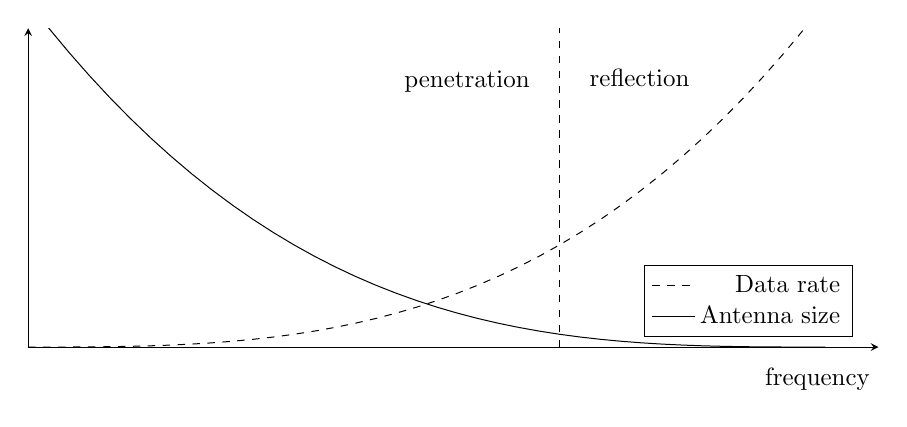
\begin{tikzpicture}[scale=0.9]
\begin{axis}[
x=1.5cm,
y=1.5cm,
axis y line=left,
axis x line=bottom,
xmax=8,xmin=0,
ymin=0,ymax=3,
xlabel=frequency,
x label style={at={(axis description cs:1,-0.1)},anchor=east},
ylabel=,
xmajorticks=false,
ymajorticks=false,
width=15cm,
anchor=center,
legend pos=south east,
legend cell align={right}
]
\addplot+ [samples = 40, domain=0:7.5, no markers, black, dashed] {x^3/130};
\addlegendentry{Data rate}
\addplot+ [samples = 40, domain=0:7.5, no markers, black] {-(x-7.5)^3/130};
\addlegendentry{Antenna size}
\addplot+ [mark=none, black, dashed] coordinates {(5, 0) (5, 3)};
\node [anchor=east] at (4.8,2.5) {penetration};
\node [anchor=west] at (5.2,2.535) {reflection};
\end{axis}
\end{tikzpicture}
\captionof{figure}{Operation frequencies}
\end{center}

\subsection{Communication, Coding and Modulation}
\begin{mytitle}[Communication principles] The field of the reader may be turned off periodically to allow transponders to send in-between. This requires a capacitor on the transponders to buffer energy.
\end{mytitle}
\begin{mytitle}[Typical encoding schemes] 
    \begin{mysubtitle}[NRZ] 1 = high, 0 = low
    \end{mysubtitle}
    \begin{mysubtitle}[Manchester] 1 = high$\to$low, 0 = low$\to$high. This is typically used for tag to reader communication.
    \end{mysubtitle}
    \begin{mysubtitle}[Pulse pause coding (PPC)] 1 = short period to next pause, 0 = long period to next pause. This is typically used for reader to tag communication.
    \end{mysubtitle}
\end{mytitle}
\begin{mytitle}[Data transfer from reader to tag] Amplitude shift keying (ASK) is used to switch the antenna driver of the reader on and off. ASK uses a finite number of amplitudes each assigned to an unique pattern of bits. The energy stored in the reader's antenna decays rapidly by cutting it down with clipping diodes. 
\end{mytitle}
\begin{mytitle}[Data transfer from tag to reader] There are several principles used here:
\begin{itemize}
    \item Capacitive coupling uses an electrical field and works for very short distances
    \item Load modulation uses a magnetic field and works for near distances. Magnetic coupling works by turning a resistor in the oscillating circuit of the transponder on and off and thus yielding a small voltage change at the antenna of the reader.
    \item Backscatter uses an electromagnetic field and works for long ranges. Electromagnetic coupling works by switching a resistor parallel to the transponder antenna on and off and thus changing the reflection properties. 
\end{itemize}
The data rate is typically several kbits/s up to 100 kbits/s.
\end{mytitle}


\subsection{Anti-Collision Protocols}
\begin{mytitle}[The collision problem] The reader broadcasts energy and its signal to many transponders, then all transponders may react simultaneously. They will interfere if there is only a single shared channel. Ideally a transponder should have exclusive access to the shared channel during the short period where it transmits a few bytes. But transponders usually don't hear the signal from other transponders, only the one from the reader. We want access control and collision detection/avoidance to be fast and reliable.
\end{mytitle}
\begin{mytitle}[Capture effect] The throughput improves if transponders closer to the reader "win" because of their stronger signal. Difference in signal strength leads to the problem of weak collisions, where the reader might not notice the presence of a weak signal because of an overwhelming presence of a strong signal and thus collisions might go unnoticed.
\end{mytitle}
\begin{mytitle}[Collision avoidance with FDMA] This approach needs many channels in parallel, hence it is only suitable for some particular applications with a small, fixed number of transponders.
\end{mytitle}
\begin{mytitle}[Stochastic protocols] Stochastic protocols usually do not detect all tags in one read cycle, there is overall less reader to tag communication and there is typically an ALOHA-based anti-collision algorithm.
    \begin{mysubtitle}[ALOHA principle] Transponders repeatedly send out their data with random length quiet periods in-between. The data should eventually get through. The higher the load, the more collisions happen. This has a maximal throughput of 18.4\%. This is a stochastic TDMA protocol.
    \end{mysubtitle}
    \begin{mysubtitle}[Slotted ALOHA] Transponders start their transmissions only at well-defined instants (slots). Synchronization is done by the reader who periodically sends out "sync" commands. All transponders then send their serial number in one of the following slots. If the reader gets only one serial number "sn", it sends a "select sn" command. Only the transponder with serial number "sn" responds by sending its payload data. The maximal throughput is then 36.8\%. 
    \end{mysubtitle}
    \begin{mysubtitle}[Reservation ALOHA] This protocol has two phases: first a short ALOHA phase where the transponders compete for reservations, then the reserved phase for payload data transmission. 
    \end{mysubtitle}
    \begin{mysubtitle}[Adaptive round algorithm] In this extension of reservation ALOHA the number of slots is dynamically altered, depending on the number of collisions and empty slots.
    \end{mysubtitle}
\end{mytitle}
\begin{center}
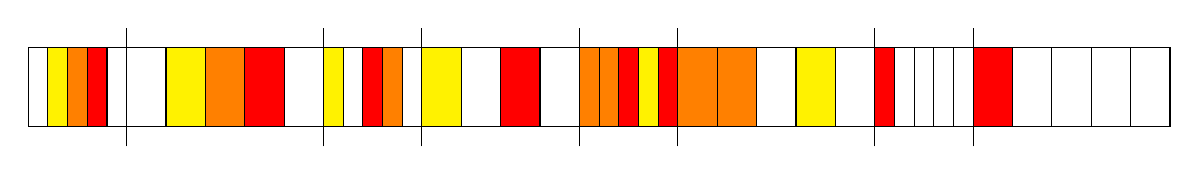
\begin{tikzpicture}[scale = 0.5]

%\draw (0, 0) rectangle (30, 2);
\draw [fill = white] (0, 0) rectangle (0.5, 2);
\draw [fill = yellow] (0.5, 0) rectangle (1, 2);
\draw [fill = orange] (1, 0) rectangle (1.5, 2);
\draw [fill = red] (1.5, 0) rectangle (2, 2);
\draw [fill = white] (2, 0) rectangle (2.5, 2);

\draw [] (2.5, -0.5) -- (2.5, 2.5);

\draw [fill = white] (2.5, 0) rectangle (3.5, 2);
\draw [fill = yellow] (3.5, 0) rectangle (4.5, 2);
\draw [fill = orange] (4.5, 0) rectangle (5.5, 2);
\draw [fill = red] (5.5, 0) rectangle (6.5, 2);
\draw [fill = white] (6.5, 0) rectangle (7.5, 2);

\draw [] (7.5, -0.5) -- (7.5, 2.5);

\draw [fill = yellow] (7.5, 0) rectangle (8, 2);
\draw [fill = white] (8, 0) rectangle (8.5, 2);
\draw [fill = red] (8.5, 0) rectangle (9, 2);
\draw [fill = orange] (9, 0) rectangle (9.5, 2) node[midway] {\Lightning}; 
\draw [fill = white] (9.5, 0) rectangle (10, 2);

\draw [] (10, -0.5) -- (10, 2.5);

\draw [fill = yellow] (10, 0) rectangle (11, 2);
\draw [fill = white] (11, 0) rectangle (12, 2);
\draw [fill = red] (12, 0) rectangle (13, 2);
\draw [fill = white] (13, 0) rectangle (14, 2);
\draw [fill = white] (14, 0) rectangle (15, 2);

\draw [] (14, -0.5) -- (14, 2.5);

\draw [fill = orange] (14, 0) rectangle (14.5, 2);
\draw [fill = orange] (14.5, 0) rectangle (15, 2);
\draw [fill = red] (15, 0) rectangle (15.5, 2) node[midway] {\Lightning}; 
\draw [fill = yellow] (15.5, 0) rectangle (16, 2);
\draw [fill = red] (16, 0) rectangle (16.5, 2) node[midway] {\Lightning}; 

\draw [] (16.5, -0.5) -- (16.5, 2.5);

\draw [fill = orange] (16.5, 0) rectangle (17.5, 2);
\draw [fill = orange] (17.5, 0) rectangle (18.5, 2);
\draw [fill = white] (18.5, 0) rectangle (19.5, 2);
\draw [fill = yellow] (19.5, 0) rectangle (20.5, 2);
\draw [fill = white] (20.5, 0) rectangle (21.5, 2);

\draw [] (21.5, -0.5) -- (21.5, 2.5);

\draw [fill = red] (21.5, 0) rectangle (22, 2);
\draw [fill = white] (22, 0) rectangle (22.5, 2);
\draw [fill = white] (22.5, 0) rectangle (23, 2);
\draw [fill = white] (23, 0) rectangle (23.5, 2);
\draw [fill = white] (23.5, 0) rectangle (24, 2);

\draw [] (24, -0.5) -- (24, 2.5);

\draw [fill = red] (24, 0) rectangle (25, 2);
\draw [fill = white] (25, 0) rectangle (26, 2);
\draw [fill = white] (26, 0) rectangle (27, 2);
\draw [fill = white] (27, 0) rectangle (28, 2);
\draw [fill = white] (28, 0) rectangle (29, 2);

\end{tikzpicture}
\captionof{figure}{Reservation ALOHA}
\end{center}
\begin{mytitle}[Deterministic protocols] Deterministic protocols usually detect all tags that are present in a read cycle, but they introduce high reader to tag communication overheads. There is typically a tree-walking anti-collision algorithm.
    \begin{mysubtitle}[Tree-walking anti-collision algorithm] \hfill
    \begin{itemize}
        \item The coding scheme: We use Manchester encoding, so that where two signals that are transmitting over each other differ, it results in an illegal signal and the reader can locate these bits. This requires bit synchronization.
        \begin{center}
\begin{tikzpicture}
\draw [black, line width=0.4mm] (0, 1) -- (0.5, 1) -- (0.5, 0) -- (1, 0) -- (1, 1);
\draw [firstAccent, line width=0.4mm] (1, 1) -- (2, 1);
\draw [black, line width=0.4mm] (2, 1) -- (2.5, 1) -- (2.5, 0) -- (3, 0) -- (3, 1);
\draw [firstAccent, line width=0.4mm] (3, 1) -- (4, 1);
\draw [black, line width=0.4mm] (4, 1) -- (4, 0) -- (4.5, 0) -- (4.5, 1) -- (5, 1);
\draw [black, line width=0.4mm] (5, 1) -- (5, 0) -- (5.5, 0) -- (5.5, 1) -- (6, 1);

\draw [black, line width=0.4mm] (0, 3) -- (0.5, 3) -- (0.5, 2) -- (1, 2) -- (1, 3);
\draw [firstAccent, line width=0.4mm] (1, 3) -- (1.5, 3) -- (1.5, 2) -- (2, 2);
\draw [black, line width=0.4mm] (2, 2) -- (2, 3) -- (2.5, 3) -- (2.5, 2) -- (3, 2);
\draw [firstAccent, line width=0.4mm] (3, 2) -- (3.5, 2) -- (3.5, 3) -- (4, 3);
\draw [black, line width=0.4mm] (4, 3) -- (4, 2) -- (4.5, 2) -- (4.5, 3) -- (5, 3);
\draw [black, line width=0.4mm] (5, 3) -- (5, 2) -- (5.5, 2) -- (5.5, 3) -- (6, 3);

\draw [black, line width=0.4mm] (0, 5) -- (0.5, 5) -- (0.5, 4) -- (1, 4);
\draw [firstAccent, line width=0.4mm] (1, 4) -- (1.5, 4) -- (1.5, 5) -- (2, 5);
\draw [black, line width=0.4mm] (2, 5) -- (2.5, 5) -- (2.5, 4) -- (3, 4) -- (3, 5);
\draw [firstAccent, line width=0.4mm] (3, 5) -- (3.5, 5) -- (3.5, 4) -- (4, 4);
\draw [black, line width=0.4mm] (4, 4) -- (4.5, 4) -- (4.5, 5) -- (5, 5);
\draw [black, line width=0.4mm] (5, 5) -- (5, 4) -- (5.5, 4) -- (5.5, 5) -- (6, 5);

\draw [black] (0, -0.2) -- (0, 5.2);
\draw [black] (1, -0.2) -- (1, 5.2);
\draw [black] (2, -0.2) -- (2, 5.2);
\draw [black] (3, -0.2) -- (3, 5.2);
\draw [black] (4, -0.2) -- (4, 5.2);
\draw [black] (5, -0.2) -- (5, 5.2);
\draw [black] (6, -0.2) -- (6, 5.2);

\node at (-0.5, 0.5) [anchor=east] {decoded signal at the reader};
\node at (-0.5, 2.5) [anchor=east] {transponder 2};
\node at (-0.5, 4.5) [anchor=east] {transponder 1};
\end{tikzpicture}
\captionof{figure}{Coding scheme to detect collisions}
\end{center}
        \item The basic idea: The reader broadcasts a "sync" to all transponders, then requests the ID number of all transponders. It then determines the leftmost bit $b$ that yields a collision. If there is none, the reader requests data from the unique transponder $x$, then sends "halt" to $x$. Then the reader moves up the tree to the next appropriate subtree with a different value of the last $b$. If there is a collision, the reader broadcasts "mute if value 0 at position $b$". Only transponders with value 1 at position $b$ move to the next round, all others remain mute from now on.
    \end{itemize}
    \end{mysubtitle}
\end{mytitle}

\begin{mytitle}[Business-relevant and application-driven criteria] \hfill
\begin{itemize}
    \item Read range: Low and high frequency have a read range of 1-1.5 m, ultra high frequency has a read range of around 10 m. The working area is typically complex.
    \item Data transfer and detection rate: Low and high frequency have a data transfer rate of 5 kb/s, ultra high frequency has a data transfer rate of 50 kb/s. The detection rate depends on the data transfer rate, the choice of anti-collision algorithm and the length of the tag ID. Typically low and high frequency have a detection rate of 10-30 tags/s, ultra high frequency has a range of 100-500 tags/s.
    \item Susceptibility to noise and other error sources: This depends on frequency, antenna size and protocol.
    \item Cost: The cost typically ranges from a few cents to a few dollars.
    \item Form factors: This includes things like the coice of paper vs. plastic.
\end{itemize}
\end{mytitle}

\subsection{Strengths and Drawbacks of RFID}
\begin{mytitle}[Strengths of RFID] \hfill
\begin{itemize}
    \item No line of sight required
    \item Longer read range
    \item More bits
    \item Multiple tags can be read nearly simultaneously
    \item Write and change data
    \item Possibility to integrate sensors
\end{itemize}
\end{mytitle}
\begin{mytitle}[Drawbacks of RFID]\hfill
\begin{itemize}
    \item Cost
    \item Unreliable under certain conditions
\end{itemize}
\end{mytitle}
